\section{Architecture GNU/Linux}

\begin{frame}{Architecture}{Système GNU/Linux}
	Linux est un noyau. Seul il ne sert à rien. On parlera donc de système GNU/Linux.
	Il est en général composé de:
	\begin{itemize}
		\item
			Un bootloader (Rare sont les carte capable de booter un noyau Linux)\\
			Il est trop gros et doit etre chargé en RAM (elle doit etre initialisé par un microcode)
		\item
			Le noyau Linux (gérant les ressources de la machine)
		\item
			Un système de fichier contenant à minima un programme de démarrage (rootfs)
	\end{itemize}
\end{frame}

\begin{frame}{Architecture}{Système GNU/Linux}
	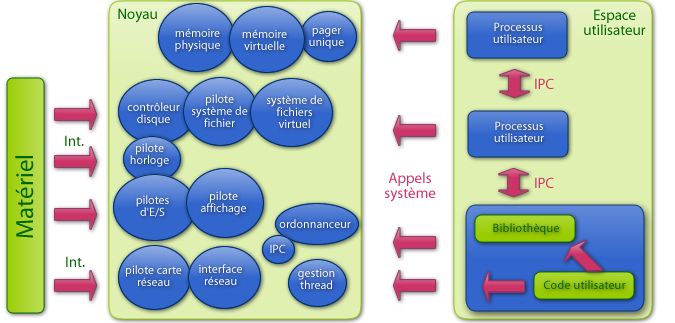
\includegraphics[width=10cm]{system_arch.png}
\end{frame}

\subsection{Noyau}
\begin{frame}{Architecture}{Noyau}
	Le noyau Linux est un binaire de type ELF.\\
	Son image est souvent compréssé pour gagner en taille lors du déploiement et de la copie en RAM\\
	Il contient un auto extracteur qui va le décomprésser\\
	Fournit des services nécéssaires à sa fonction:
	\begin{itemize}
		\item
			ordonanceur
		\item
			gestion mémoire, disque, interface réseaux
		\item
			service abtraits (systeme de fichier, pile réseaux ...)
	\end{itemize}
	Une grande partie du noyau peut etre déporté en module chargé dynamiquement.
\end{frame}

\begin{frame}{Architecture}{Noyau}
	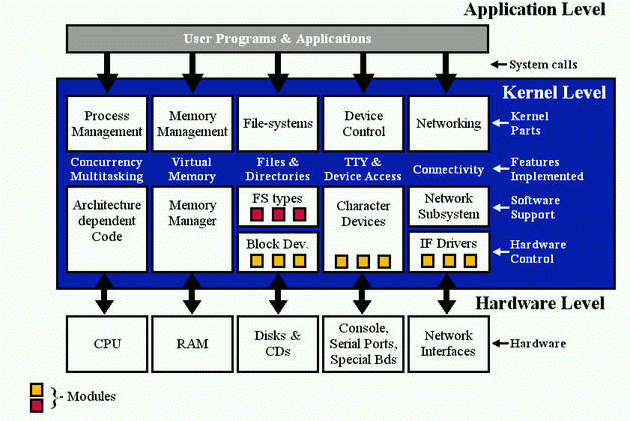
\includegraphics[width=10cm]{kernel_arch.png}
\end{frame}

\begin{frame}{Architecture}{Module noyau}
	Modules noyau: .ko (Kernel Object)\\
	Les modules binaires sont liés à la version du noyau !\\
	Peut se compiler après Nécéssite les entetes du noyau\\
	Mécanisme système pour charger les modules dynamiquement: modprobe, insmod, rmmod
\end{frame}

\subsection{Rootfs}

\begin{frame}{Architecture}{Organisation d'un rootfs}
	Organisation commune à 90\% entre les UNIX
	Quelques spécificités GNU/Linux et distribution
	Les fichiers communs:
	\begin{itemize}
		\item
			/bin,/sbin,/usr/bin,/usr/sbin: binaires communs et systèmes
		\item
			/lib,/usr/lib: bibliothèques et modules noyau
		\item
			/etc: fichiers de configuration
		\item
			/dev: nœuds d'accès aux périphériques (nodes)
		\item
			/var: fichiers variables: log, spool, mail, ...
		\item
			/opt: pour les programmes externes (ex: OpenOffice)
		\item
			/home: accueille les répertoires des utilisateurs
	\end{itemize}
\end{frame}

\begin{frame}{Architecture}{Organisation d'un rootfs}	
	Quelques répertoires spéciaux:
	\begin{itemize}
		\item
			/lib/modules: contient les modules du noyau
		\item
			/root: home-directory de l'utilisateur root (pas dans OE)
		\item
			/media: point de montage des volumes amovibles
		\item
			/proc: système de fichier virtuel (état du système)
		\item
			/sys: idem pour les périphériques connectés (2.6)
		\item
			/boot: noyau statique (vmlinuz, uImage, ...)
	\end{itemize}
\end{frame}

\begin{frame}{Architecture}{/proc}
	Système de fichier virtuel (lecture/écriture) géré par le noyau. (Réponse sur solicitation, pas d'écriture sur un support)\\
	Intérêt: manipuler les variables systèmes comme de fichiers (cat, echo, grep)\\
	Exemples:
	\begin{itemize}
		\item
			/proc/version: version du noyau
		\item
			/proc/cpuinfo: type(s) de processeur(s)
		\item
			/proc/interrupts: interruptions
		\item
			/proc/pid: répertoire décrivant le processus associé au pid
		\item
			/proc/mounts: partitions montées
		\item
			/proc/modules: liste des modules noyau chargés
	\end{itemize}
	Nombreuses commandes systèmes basé sur /proc : lsmod, lspci, top, mount, ...
	Il est aisé de proposer une entrée dans /proc dans un nouveau module grâce à une API
\end{frame}

\begin{frame}{Architecture}{/sys}
	Introduit dans le noyau 2.6 (2003) => sysfs\\
	Vue synthétique des périphériques connectés\\
	\begin{itemize}
		\item
			/sys/class (utilisé par UDEV)
		\item
			/sys/modules
		\item
			/sys/bus
	\end{itemize}		
	But: mieux gérer l'ajout/suppression dynamique des périphériques (hotplug)
	Utilisé par UDEV pour créer dynamiquement les entrées dans /dev 
	Quelques recouvrements avec /proc (bus PCI, USB, ...)
\end{frame}